\documentclass[a4paper, 10pt, final, garamond]{book}
\usepackage{cours-preambule}

\makeatletter
\renewcommand{\@chapapp}{Thermodynamique -- chapitre}
\makeatother

\hfuzz=5.002pt

% \toggletrue{student}
% \toggletrue{corrige}
% \renewcommand{\mycol}{black}
% \renewcommand{\mycol}{gray}

\begin{document}
\setcounter{chapter}{1}

\settype{enon}
\settype{solu_prof}
\settype{solu_stud}

\chapter{\cswitch{Correction du TD}{TD~: Échanges d'énergie des systèmes
	  thermodynamiques}}

\resetQ
\section[s]"1"{Transformations de tous les jours}
\enonce{%
	Caractérisez les transformations thermodynamiques suivantes~:
}%

\QR{%
	Vous placez dans un thermos du thé bouillant et de l'eau froide.
}{%
	Transformation adiabatique d'une phase condensée, isobare et isochore( et
	monotherme, mais inutile si pas d'échange de chaleur).
}%
\QR{%
	Vous oubliez votre tasse de café dans la cuisine la journée.
}{%
	Transformation monotherme, isobare et isochore.
}%

\resetQ
\section[s]"1"{Travail reçu le long d'un chemin donné}
\enonce{%
	Un système constitué de $n$ moles de gaz parfait subit une transformation d'un
	état initial A $(P_1 = \SI{4.0}{bar}, V_1 = \SI{10}{L}, T_1 = \SI{600}{K})$
	vers un état final B $(P_2 = \SI{1.0}{bar}, V_2 = \SI{20}{L}, T_2)$.
}%
\QR{%
	Déterminer $T_2$.
}{%
	\leavevmode\vspace*{-15pt}\relax
	\begin{gather*}
		\beforetext{Le gaz étant parfait,}
		P_1V_1 = nRT_1
		\qet
		P_2V_2 = nRT_2
		\\\Lra
		n = \frac{P_1V_1}{RT_1}
		\qet
		\boxed{T_2 = \frac{P_2V_2}{P_1V_1}T_1}
		\\\Ra
		\xul{T_2 = \SI{300}{K}}
	\end{gather*}
}%
\QR{%
	Cette transformation est constituée de deux étapes~: une transformation
	isobare de A vers C puis une transformation isochore de C vers B. Déterminer
	le travail $W\ind{AB}$.
}{%
	$W\ind{AB} = W\ind{AC} + W\ind{CB}$.
	\begin{itemize}
		\item $W\ind{CB} = 0$ car isochore~;
		      \item[m][25]
		      \begin{gather*}
			      \beforetext{Si $A \ra C$ quasi-statique,}
			      W\ind{AC} = - \int_{A}^{C} P \dd{V}
			      \\\beforetext{Comme $A \ra C$ isobare, $P = P_1$ et}
			      W\ind{AC} = -P_1 (V_2-V_1)
		      \end{gather*}
	\end{itemize}
	\begin{gather*}
		\beforetext{Ainsi,}
		W\ind{AB} = W\ind{AC}
		\Ra
		\xul{W\ind{AB} = \SI{-4.0}{kJ}}
	\end{gather*}
}%
\QR{%
	On considère un autre chemin~: une transformation isochore de A vers D puis
	une transformation isobare de D vers B. Déterminer le travail $W\ind{AB}$.
}{%
	De même que précédemment, la transformation isochore a un travail nul, donc
	seule la transformation de D vers B travaille, et $W\ind{AB} = W\ind{DB}$.
	Seulement, la pression de l'isobare n'est plus la même, et on trouve
	\[
		W\ind{AB} = W\ind{DB} = -P_2 (V_2-V_1)
		\\\Ra
		\xul{W\ind{AB} = \SI{-1.0}{kJ}}
	\]
}%
\QR{%
	Représenter ces deux transformations sur un schéma et retrouver graphiquement
	quelle transformation a le plus grand travail et le signe dudit travail.
}{%
	\noindent
	\begin{minipage}[t]{.30\linewidth}
		\vspace{0pt}
		\begin{center}
			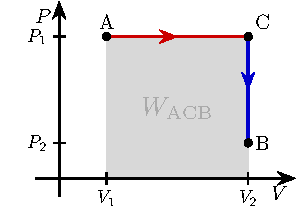
\includegraphics[width=\linewidth]{isoP-isoV}
		\end{center}

	\end{minipage}
	\hfill
	\begin{minipage}[t]{.30\linewidth}
		\vspace{0pt}
		\begin{center}
			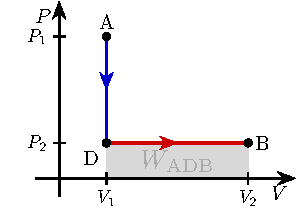
\includegraphics[width=\linewidth]{isoV-isoP}
		\end{center}
	\end{minipage}
	\hfill
	\noindent
	\begin{minipage}[t]{.30\linewidth}
		\vspace{0pt}
		L'aire sous la courbe est en effet plus grande pour la transformation ACB.
		On voit que le signe est négatif puisqu'on parcours le trajet dans le sens
		horaire.
	\end{minipage}
}%

\resetQ
\section[s]"1"{Diagramme de \textsc{Clapeyron}}
\enonce{%
	Considérons un système fermé qui subit une transformation d'un état
	d'équilibre initial $(P_i, V_i)$ à un état d'équilibre final $(P_f, V_f)$, de
	manière mécaniquement réversible.
}%
\QR{%
	Représenter les différentes transformations dans un diagramme de
	\textsc{Clapeyron} $(P,v)$~: isochore, isobare, isotherme d'un gaz parfait,
	adiabatique d'un gaz parfait, caractérisée par $PV^{\gamma} = \cte$
	avec $\gamma > 1$.
}{%
	\sswitch{
		\hfill
		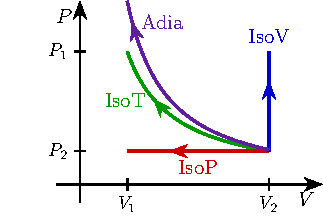
\includegraphics[width=.5\linewidth, valign=t]{PV_all}
		\hspace*{\fill}
	}{
		\begin{center}
			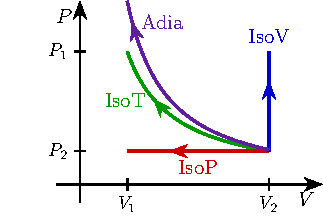
\includegraphics[width=.5\linewidth]{PV_all}
		\end{center}
	}
}%
\QR{%
	Faire le lien entre l'aire sous la courbe et le travail des forces de
	pression dans ce diagramme.
}{%
	\leavevmode\vspace*{-25pt}\relax
	\begin{gather*}
		\Ac =
		\int_{v_i}^{v_f} P \dd{v} =
		-\frac{1}{m} \left( - \int_{V_i}^{V_f} P \dd{V} \right)
		\\\beforetext{Or $P = P\ind{ext}$ pour quasi-statique}
		\boxed{\Ac = - \frac{W_p}{m}}
	\end{gather*}
}%
\QR{%
	Pour une transformation cyclique, faire le lien entre le sens de parcours du
	cycle et le signe du travail au cours d'un cycle.
}{%
	$\dd{V} > 0 \Lra W_p < 0$ et inversement. Or, si le cycle est parcouru dans le
	\textbf{sens direct}, alors la transformation de $\dd{V} > 0$ passe en-dessous
	de la transformation de $\dd{V} < 0$~; ainsi l'aire entourée correspond à un
	travail \textbf{positif}.
	\begin{center}
		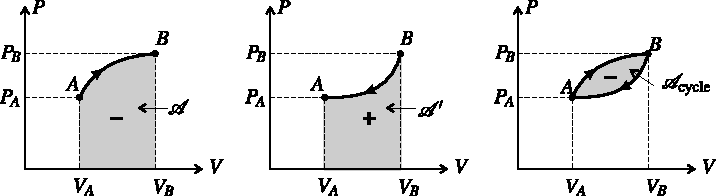
\includegraphics[width=.8\linewidth]{W_cycle-demo}
	\end{center}
}%

\resetQ
\section[s]"2"{Calculs de travaux et transferts thermiques}
\enonce{%
On considère trois moles de dioxygène, gaz supposé parfait, qu'on peut faire
passer de l'état initial A $(P_A, V_A, T_A)$ à l'état final B $(P_B, V_B,
	T_B)$ par trois transformations distinctes~:
\begin{itemize}
	\item A1B isotherme~;
	\item A2B représentée par une droite dans le diagramme $(P,V)$~;
	\item A3B composée d'une transformation à pression constante, suivie d'une
	      transformation à volume constant.
\end{itemize}
On considère l'équilibre thermodynamique interne conservé à tout instant. On
donne $P_B = 3 P_A$, $T_A = \SI{300}{K}$ et $R =
	\SI{8.314}{J.K^{-1}.mol^{-1}}$.
}%
\QR{%
	Représenter les trois transformations dans le diagramme $(P,V)$.
}{%
	\sswitch{
		\hfill
		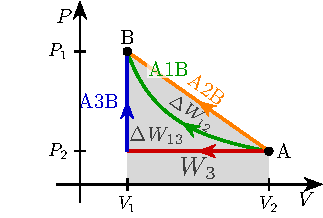
\includegraphics[width=.5\linewidth, valign=t]{PV_droite}
		\hspace*{\fill}
	}{
		\begin{center}
			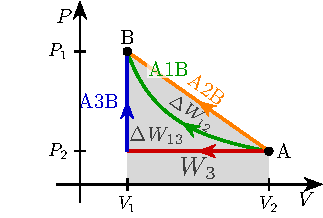
\includegraphics[width=.5\linewidth]{PV_droite}
		\end{center}
	}
}%
\QR{%
	Déterminer la température $T_B$ et le volume $V_B$.
}{%
	\begin{itemize}
		\item A et B sont reliés par une isotherme, donc $\boxed{T_A = T_B =
				      \SI{300}{K}}$.
		\item
		      \leftcenters{%
			      On a donc $P_AV_A = P_BV_B$, soit
		      }{%
			      $\boxed{\DS V_B = V_A \frac{P_A}{P_B} = \frac{V_A}{3}}$
		      }%
	\end{itemize}
}%
\QR{%
	Exprimer les travaux reçus par le système pour ces trois transformations.
	Commentez.
}{%
	On condidère les transformations comme quasi-statique, soit $\boxed{P =
			P\ind{ext}}$. Ainsi~:
	\begin{gather*}
		\beforetext{A1B~:}
		W_1 = -\int_{A}^{B} P \dd{V} = -nRT_A \ln \frac{V_B}{V_A}
		\Lra
		\boxed{W_1 = P_AV_A \ln 3}
		\\\beforetext{A2B~:}
		W_2 = W\ind{rect} + W\ind{trgl} = P_A(V_B-V_A) + \frac{1}{2} (P_B - P_A)(V_B
		- V_A)
		\Lra
		\boxed{W_2 = \frac{4}{3}P_AV_1}
		\\\beforetext{A3B~:}
		W_3 = -P_A(V_B - V_A)
		\Lra
		\boxed{W_3 = \frac{2}{3}P_AV_A}
	\end{gather*}
	Le travail des forces de pression dépend ainsi du chemin suivi.
}%
\QR{%
	Exprimer les transferts thermiques reçus par le système pour ces trois
	transformations. On donne le premier principe de la thermodynamique~:
	$\Delta{U} = W + Q$.
}{%
	Comme $T_A = T_B$, on a $\Delta{U} = 0$. Avec le premier principe~:
	\[
		\boxed{Q = -W}
	\]
}%

\resetQ
\section[s]"3"{Étude d'un compresseur}
\enonce{%
	\noindent
	\begin{minipage}[c]{.48\linewidth}
		On s'intéresse au compresseur d'un moteur à air comprimé, comme celui d'un
		marteau-piqueur par exemple. L'air est assimilé à un gaz parfait. Il est
		aspiré dans les conditions atmosphériques, sous la pression $P_0 =
			\SI{1}{bar}$ et à la température $T_0 = \SI{290}{K}$, jusqu'au volume $V_m$.
		Il est ensuite comprimé jusqu'à la pression $P_1$ où il occupe un volume
		$V_1$, et est refoulé à la température $T_1$ dans un milieu où la pression
		est $P_1 = \SI{6}{bar}$.
	\end{minipage}
	\hfill
	\begin{minipage}[c]{.48\linewidth}
		\begin{center}
			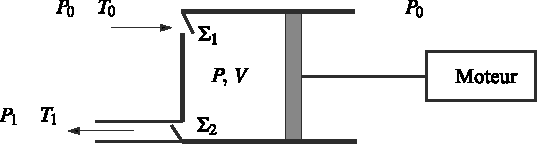
\includegraphics[width=\linewidth]{compresseur-plain}
		\end{center}
	\end{minipage}
	Bien que le mécanisme réel d'un compresseur soit
	différent, on suppose que celui-ci fonctionne comme une pompe à piston, qui se
	compose d'un cylindre, d'un piston coulissant entraîné par un moteur et de
	deux soupapes~:
	\begin{itemize}
		\item La soupape d'entrée $\Sigma_1$ est ouverte si la pression $P$ dans le
		      corps de la pompe est inférieure ou égale à la pression atmosphérique
		      $P_0$~;
		\item La soupape de sortie $\Sigma_2$ est ouverte si $P$ est supérieure à
		      $P_1$~;
		\item Le volume $V$ du corps de pompe est compris entre $0$ et $V_m$~;
		\item À chaque cycle (un aller-retour du piston), la pompe aspire et refoule
		      une mole d'air.
	\end{itemize}
}%
\begin{blocQR}
	\item
	\QR{%
		Tracer sur un diagramme de \textsc{Watt} $(P,V)$ l'allure de la courbe
		représentant un aller-retour du piston. Indiquer le sens de parcours par une
		flèche.
	}{%
		\noindent
		\begin{minipage}[t]{.55\linewidth}
			On étudie le gaz qui entre dans le corps de la pompe pendant la première
			phase. L'évolution étudiée comporte les trois étapes suivantes~:
			\begin{enumerate}[label=\clenumi]
				\item Admission du gaz de A à B à la pression $P_0$~;
				\item Compression de B à C~;
				\item Refoulement de C à D à la pression $P_1$.
			\end{enumerate}
		\end{minipage}
		\hfill
		\begin{minipage}[t]{.40\linewidth}
			\vspace{0pt}
			\begin{center}
				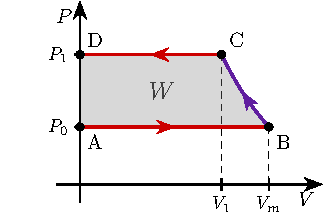
\includegraphics[width=\linewidth]{PV_compresseur}
			\end{center}
		\end{minipage}
	}%
	\QR{%
		Montrer que le travail de l'air situé à droite du piston est nul sur un
		aller-retour.
	}{%
		La pression extérieure est constante, donc le travail des forces de pression
		du gaz à droite du piston est~:
		\[
			W\ind{droite} =
			W\ind{droite,AB} + W\ind{droite,BC} + W\ind{droite,CD} =
			P_0 (
			\cancel{V_B} - \bcancel{V_A} +
			\dcancel{V_C} - \cancel{V_B} +
			\bcancel{V_D} - \dcancel{V_C}
			) = 0
		\]
		En effet, puisque le piston effectue un aller-retour, le volume balayé est
		le même à l'aller (travail résistant) qu'au retour (travail moteur).
	}%
	\QR{%
		Montrer que le travail fourni par le moteur qui actionne le piston est égal
		à l'aire d'une surface sur le diagramme. On supposera que le mouvement est
		assez lent pour que l'évolution soit mécaniquement réversible.
	}{%
		La force exercée par le moteur pour déplacer le piston est $F = (P-P_0)S$
		avec $S$ la section du piston. Ainsi, le travail \textbf{reçu} par le moteur
		est~:
		\[
			W\ind{moteur}\sup{reçu} =
			\int_{\mathrlap{ABCD}} ~~ (P - P_0)\dd{V} =
			\int_{\mathrlap{ABCD}} ~~ P \dd{V} - W\ind{droite}
			\Lra
			\boxed{W\ind{moteur}\sup{fourni} = -\int_{\mathrlap{ABCD}} ~~ P \dd{V}}
		\]
		En effet, le travail \textbf{fourni par le moteur} est l'opposé de son
		travail reçu, et est égal au travail \textbf{reçu par le gaz}, en supposant
		la pression $P$ définie à chaque instant. C'est ce qu'on appelle
		habituellement le travail de l'opérataire.
	}%
\end{blocQR}
\QR{%
Pendant la phase de compression, l'air suit une loi polytropique $PV^k =
	\cte$. Il sort du compresseur à la température $T_1 = \SI{391}{K}$. Trouver la
valeur de $k$.
}{%
On étudie le gaz entre B et C. On retrouve une expression proche de la loi de
\textsc{Laplace}, et on connaît $P$ et $T$ aux instants initial et final~: on
la convertit donc en $P^{1-\gamma}T^{\gamma} = \cte$, d'où
\begin{DispWithArrows*}[groups]
	% P_BV_m = nRT_B
	% \qqet
	% P_CV_C &= nRT_C
	% \qqet
	% P_BV_B^{k} = P_CV_C^{k}
	% \\\Ra
	%   \left( \frac{P_C}{P_B} \right) &= \left( \frac{V_B}{V_C} \right)^{k}
	%   \Arrow{}
	% & \Lra
	\left( \frac{P_C}{P_B} \right)^{1-k} &= \left( \frac{T_B}{T_C} \right)^{-k}
	\CArrow{$\ln (~\cdot~)$}
	\\
	k =
	\frac{\ln \frac{P_B}{P_C}}{\ln \frac{P_B}{P_C} - \ln \frac{T_B}{T_C}}
	&\Lra
	\boxed{k = \frac{\ln \frac{P_0}{P_1}}{\ln \frac{P_0}{P_1} - \ln \frac{T_0}{T_1}}}
	\Ra
	\xul{k = \num{1.2}}
\end{DispWithArrows*}
}%
\QR{%
	Exprimer le travail mécanique $W\ind{moteur}$ fourni par le moteur pendant un
	aller-retour en fonction de $n, R, k, T_1$ et $T_0$.
}{%
	On calcule le travail sur les trois transformations élémentaires~:
	\begin{enumerate}[label=\clenumi]
		\item
		      \leftcenters{%
			      $P = P_0 = \cte$, donc
		      }{%
			      $
				      W\ind{AB} = -P_0 \int_{V_0}^{V_m}\dd{V} = -P_0V_m
				      \Lra
				      \boxed{W\ind{AB} = -nRT_0}
			      $
		      }%
		\item $PV^k = \cte = P_0V_m^k$, d'où
		      \leavevmode\vspace*{-30pt}\relax
		      \begin{DispWithArrows*}
			      W\ind{BC} &=
			      - \int_{V_m}^{V_1} P_0V_m^k \cdot \frac{\dd{V}}{V^k}
			      \Arrow{$\DS \int \frac{1}{V^k} \qav k>1$}
			      \\\Lra
			      W\ind{BC} &=
			      \frac{P_0V_m^{k+1-1}}{k-1} \left[ V^{1-k} \right]_{V_m}^{V_1}
			      \Arrow{On factorise par $V_m^{1-k}$}
			      \\\Lra
			      W\ind{BC} &= \frac{P_0V_m}{k-1} \left( \left( \frac{V_1}{V_m}
				      \right)^{1-k} - 1 \right)
			      \Arrow{$PV^k = \cte \Lra TV^{k-1} = \cte$\\
				      $\Lra\DS \left( \frac{V_1}{V_m}\right)^{1-k} = \frac{T_1}{T_0}$}
			      \\\Lra
			      \Aboxed{W\ind{BC} &= \frac{P_0V_m}{k-1} \left( \frac{T_1}{T_0} - 1 \right)}
		      \end{DispWithArrows*}
		\item
		      \leftcenters{%
			      $P = P_1$ donc
		      }{%
			      $
				      W\ind{CD} = -\int_{V_1}^{0}P_1 \dd{V} = P_1V_1
				      \Lra
				      \boxed{W\ind{CD} = nRT_1}
			      $
		      }%
	\end{enumerate}
	\leavevmode\vspace*{-25pt}\relax
	\begin{gather*}
		\beforetext{D'où par somme}
		\boxed{W\ind{moteur} = \frac{k}{k-1}nR (T_1-T_0)}
	\end{gather*}
}%
\QR{%
	Le débit massique de l'air dans le compresseur est $D_m =
		\SI{0.013}{kg.s^{-1}}$. Calculer la puissance $\Pc\ind{moteur}$ fournie par le
	moteur.
}{%
	Par définition, $W\ind{moteur} = \Pc\ind{moteur}\Delta{t}$. Aussi, en
	$\Delta{t} = \SI{1}{s}$ on a $n = \frac{D_m\Delta{t}}{M}$ quantité d'air
	passant dans le compresseur. Ainsi,
	\[
		\boxed{\Pc\ind{moteur} = \frac{k}{k-1} \frac{D_m}{M}R (T_1-T_0)}
		\Ra
		\xul{\Pc\ind{moteur} = \SI{2.26}{kW}}
	\]
}%

\resetQ
\section[s]"2"{Apport d'énergie électrique}
\enonce{%
	Un récipient de volume $2V_0 = \SI{4.0}{L}$ est partagé en deux compartiments
	(1) et (2), séparés par une paroi mobile et athermane. Le premier compartiment
	est calorifugé, le second est entouré de parois diathermes. Chacun contient
	$n$ moles d'un gaz parfait diatomique, qui occupe un volume initial $V_0$ sous
	la pression $P_0 = \SI{1.0}{bar}$ et la température $T_0 = \SI{300}{K}$,
	température de l'air extérieur.
	\bigbreak
	Dans le compartiment (1) se trouve une résistance électrique $R$, dans
	laquelle on fait passer un courant $I$. Le phénomène, assez lent, conduit au
	bout d'un temps $\tau$ à obtenir une pression dans le compartiment (1) telle
	que $P_1 = 2P_0$.
}%
\QR{%
	Déterminer et calculer les grandeurs $P_2$, $V_2$ et $T_2$ au bout du temps
	$\tau$ dans le compartiment.
}{%
  % TODO: Refaire schéma avec wavy line pour Q et surtout pas d'échange paroi
  % mobile !
	\begin{itemize}
		\item Équilibre mécanique et paroi mobile verticale donc $\boxed{P_2 = P_1 =
				      2P_0}$~;
		\item Évolution lente donc transfert thermiques terminés, soit $\boxed{T_2 =
				      T_0 = \SI{300}{K}}$~;
		\item Ainsi $V_2 = \frac{nRT_2}{P_2} \Lra \boxed{V_2 = \frac{V_0}{2}} =
			      \xul{\SI{1.0}{L}}$.
	\end{itemize}
	\begin{center}
		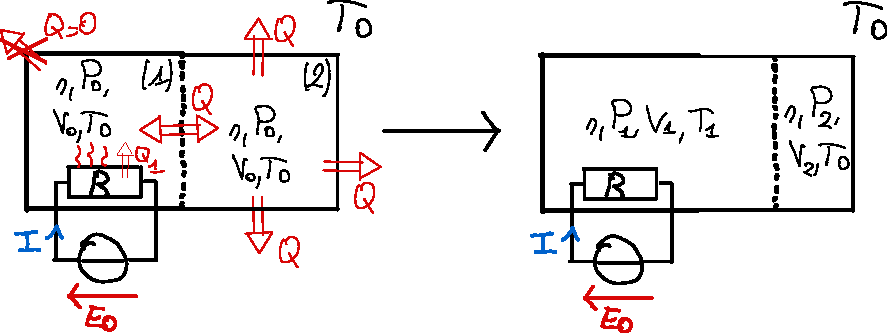
\includegraphics[width=.8\linewidth]{Q_resist}
	\end{center}
}%
\QR{%
	En déduire les expressions et les valeurs de $V_1$ et de $T_1$.
}{%
	\begin{itemize}
		\item Conservation du volume~: $V_1+V_2 = 2V_0 \Lra \boxed{V_1 = 3V_0/2} =
			      \xul{\SI{3.0}{L}}$~;
		\item $T_1 = \frac{P_1V_1}{nR} - \frac{P1V_1}{P_0V_0}T_0 \Lra \boxed{T_1 =
				      3T_0} = \xul{\SI{900}{K}}$
	\end{itemize}
}%
\QR{%
	Déterminer et calculer les variations d'énergie interne $\Delta{U_1}$ et
	$\Delta{U_2}$.
}{%
	\leavevmode\vspace*{-25pt}\relax
	\begin{gather*}
		\beforetext{Gaz de gauche}
		\Delta{U_1} = C_V\Delta{T} = \frac{5}{2}nR (T_1-T_0)
		\Lra
		\boxed{\Delta{U_1} = \frac{5}{2}\frac{P_0V_0}{T_0}(T_1-T_0)}
		\Ra
		\xul{\Delta{U_1} = \SI{1.0}{kJ}}
		\\\beforetext{Gaz de droite}
		\Delta{T}\ind{droite} = 0 \Lra \boxed{\Delta{U_2} = 0}
	\end{gather*}
}%
\QR{%
	Quel travail $W_{p,2}$ a été reçu par le compartiment (2)~? Combien vaut
	$W_{p,1}$ reçu par le compartiment (1)~?
}{%
	Transformation lente donc quasi-statique, donc $P$ compartiment 1 défini à
	chaque instant~:
	\begin{gather*}
		W_2 =
		-\int_{V_i}^{V_f} P \dd{V} =
		-nRT_0 \int_{V_i}^{V_f} \frac{\dd{V}}{V}
		\Lra
		\boxed{W_2 = P_0V_0 \ln \frac{V_0}{V_2}}
		\Ra
		\xul{W_2 = \SI{70}{J}}
		\\\beforetext{Travail reçu = $-$travail fourni donc}
		\Lra
		\boxed{W_1 = -W_2}
	\end{gather*}
}%
\QR{%
	Comment s'exprime l'énergie thermique reçue par le compartiment (1)~? La
	relier à $U$ et $W_{p,1}$ grâce au premier principe $\Delta{U} = W + Q$.
	Déterminer alors la valeur de $\tau$.
}{%
	L'énergie thermique est la puissance par effet \textsc{Joule} que multiplie le
	temps de chauffe, soit
	\[
		Q_1 = RI^2 \times \tau
		\Lra
		\boxed{\tau = \frac{\Delta{U_1}-W_1}{RI^2}}
		\Ra
		\xul{\tau = \SI{43}{s}}
	\]
}%

\end{document}
